In the dynamic analysis the hostnames was reported. The application has many external dependencies, but the domain we are interested in is, \textit{api.guloggratis.dk}. This is the api responsible of the business logic and data. The server's TLS configuration is analyzed with \href{https://www.ssllabs.com}{Qualys SSL Labs}\footnote{\href{https://www.ssllabs.com}{https://www.ssllabs.com}}. The overview can be seen on figure \ref{fig:sslreport-overview}. It is seen the server supports old version of TLS, weak ciphers and handshakes. The certificate is issued by Cloudflare and is only domain validated. Meaning it only proves they are the owner of the site but there is no organization information required to achieve such a certificate.  

\begin{figure}[htbp]
    \centering
    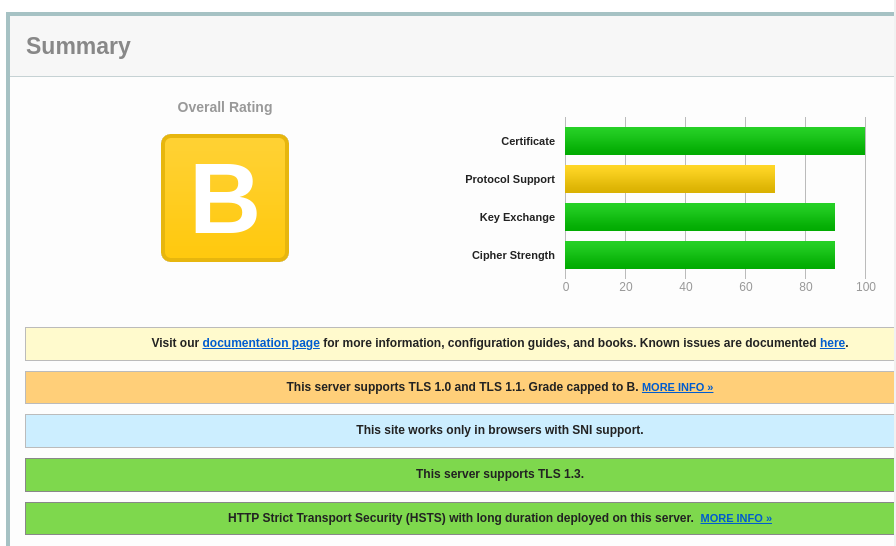
\includegraphics[width=1\columnwidth]{../static-analysis/pictures/sslreport_overview.png}
    \caption{TLS configuration of server}
    \label{fig:sslreport-overview}
\end{figure}

An attempt of performing a man-in-the-middle attack will be conducted. This revolves around setting us between the application and the server which it is communicating with. This was already performed in the dynamic analysis using MobSF. Instead of using MobSF we will do the instrumentation and configuration ourselves to fully understand the behaviour. The setup consists with the same emulator as before but now with Burp Suite as the proxy. Firstly we install the apk, disable data and proxy the wifi to Burp Suite. Then the app is started and results in the TLS connection establishment failing. This is because the phone does not trust Burp Suite's certificate. The certificate is then installed in the emulators trust store. Then traffic can be intercepted in the emulators browser but the TLS connection still fails in the application. This is caused by TLS Pinning / Certificate transparency. Remembering from the static analysis MobSF showed that this was present. Delving into the decompiled code it is seen that certificate transparency is used for the main server. The code can be seen on figure \ref{fig:retrofit-ct}

\begin{figure}[htbp]
    \centering
    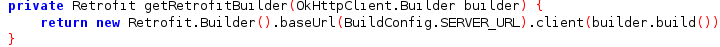
\includegraphics[width=1\columnwidth]{../static-analysis/pictures/retrofit-okkhtp-builder.png}
    \caption{Retrofit builder implementing CT with okhttp}
    \label{fig:retrofit-ct}
\end{figure}

It is not apparent that certificate transparency is implemented here. However building Retrofit on top of OkHttp activates certificate transparency\cite{android-certificate-transparency}. Thus some bypassing is necessary. It is unclear how MobSF performed this bypass, but it used \href{https://frida.re/docs/android/}{Frida}\footnote{\href{https://frida.re/docs/android/}{https://frida.re/docs/android/}}, which has several tools for this purpose. We will instead try with a patched apk generated from \href{https://github.com/shroudedcode/apk-mitm}{apk-mitm}\footnote{\href{https://github.com/shroudedcode/apk-mitm}{https://github.com/shroudedcode/apk-mitm}}. Success, it is now possible to intercept traffic in Burp Suite. The generated request from the dynamic analysis is then sent to Burp Suite for extra foundation. Multiple execution flows are performed. The traffic is then investigated. An overview of some requests can be seen on figure \ref{fig:http-requests-modules}    

\begin{figure}[htbp]
    \centering
    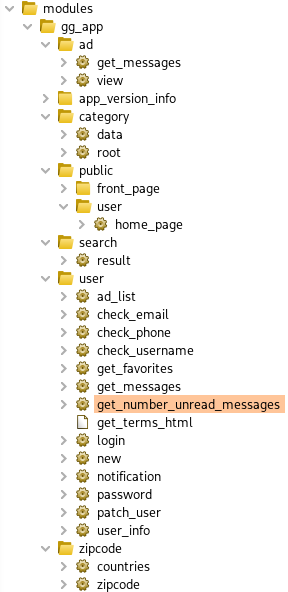
\includegraphics[width=0.5\columnwidth]{../dynamic-analysis/pictures/http-requests-modules.png}
    \caption{HTTP Requests for $<$hostname$>$/modules/}
    \label{fig:http-requests-modules}
\end{figure}

Having the setup running it is now possible to perform an attack. Looking at the example of setting an item for sale. We know by analyzing the code and requests we want to intercept \textit{modules/gg\_app/ad/} requests. The interception can be seen on figure \ref{fig:attack-new-ad}. The headline and description is than changed to \textit{mitm}. The resulting item can be seen on figure \ref{fig:attack-final-ad}.  

\begin{figure}[htbp]
    \centering
    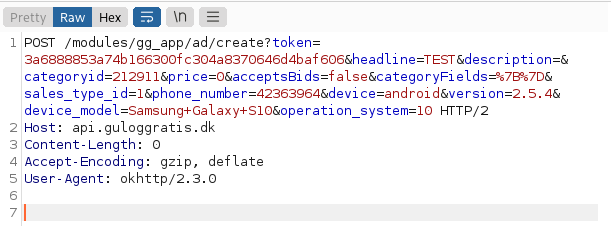
\includegraphics[width=0.5\columnwidth]{../dynamic-analysis/pictures/MITM-auction-burp.png}
    \caption{Create new ad request}
    \label{fig:attack-new-ad}
\end{figure}

\begin{figure}[htbp]
    \centering
    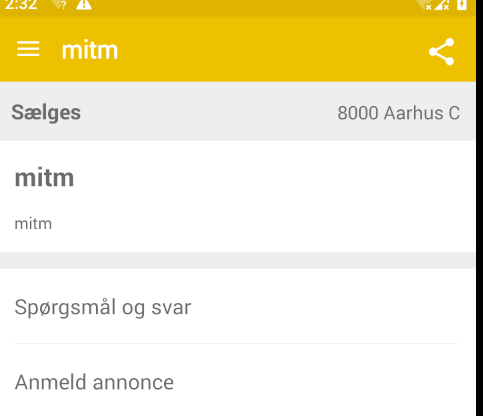
\includegraphics[width=0.5\columnwidth]{../dynamic-analysis/pictures/mitm_auction.png}
    \caption{Manipulated final item}
    \label{fig:attack-final-ad}
\end{figure}

This is an example of manipulating the requests moving from client to server. Burp Suite allow us to also manipulate the response. A result of this can be seen on figure \ref{fig:server-client-mitm}. Here the json received from server is manipulated.  

\begin{figure}[htbp]
    \centering
    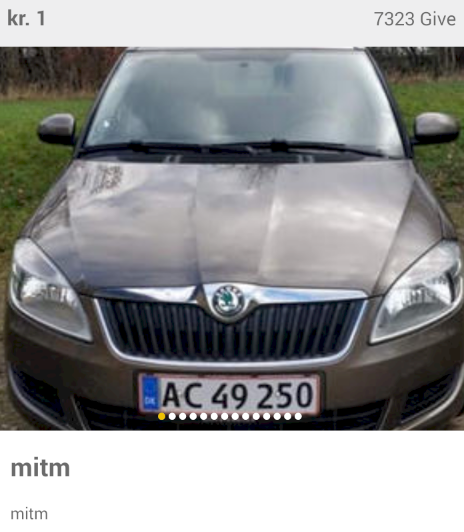
\includegraphics[width=0.5\columnwidth]{../dynamic-analysis/pictures/server-client-mitm.png}
    \caption{Manipulated response from server}
    \label{fig:server-client-mitm}
\end{figure}

In general the networking between application and server is quite easy to understand. It is not a standard REST api which follows all the standards. It is routed by \textit{modules/gg\_app/$<$entity$>$/$<$action$>$}. An example can be seen for the \textit{ad} entity on figure \ref{fig:ad-actions}. 

\begin{figure}[htbp]
    \centering
    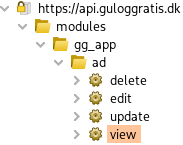
\includegraphics[width=0.5\columnwidth]{../dynamic-analysis/pictures/ad-actions.png}
    \caption{Example of actions for the ad entity}
    \label{fig:ad-actions}
\end{figure}

The HTTP methods are not used as expected. An example is that deleting an ad is done with a GET request. In general the nature of the traffic is the application targeting an action with some query parameters and then the server returning some JSON.    